%! TEX root = **/010-main.tex
% vim: spell spelllang=en:

\section{Comparison}%
\label{sec:comparison}

% Comparison and discussion of results of the different data mining methods on the validation data-set.
% Which is the best method when testing on the validation data set?  Write a comparative table.
% Try to compare different methods using McNemar test or at least show the interval of confidence for each method.
% Is there an explanation for those results (some hypothesis applicable,  etc.)? 
% Are in general accuracy on validation data set similar to the obtained with cross-validation?   
% Are  there  for  some  methods  huge  differences? If  that’s  the  case,why do you think that happens?
% Final personal evaluation of which is the best method you consider and why.

\begin{figure}[H]
\centering
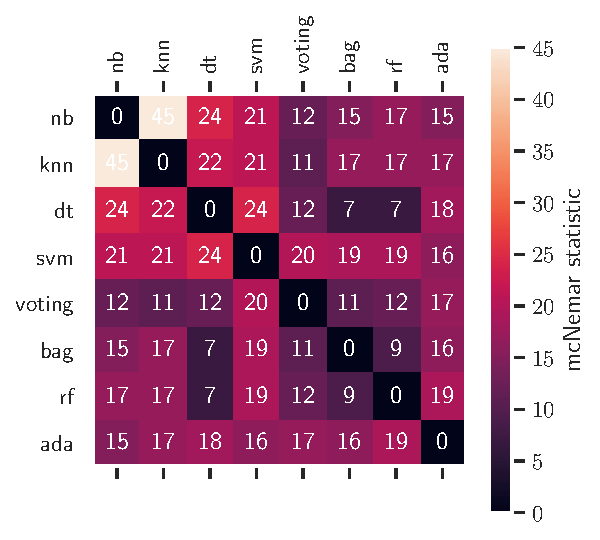
\includegraphics{mcnemar}
\end{figure}

\begin{figure}[H]
\centering
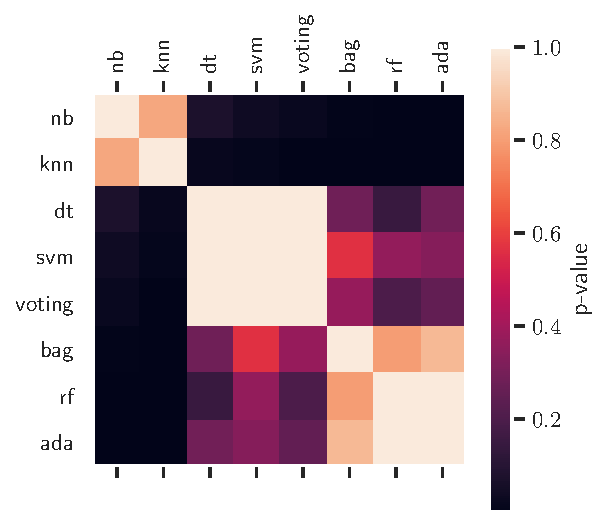
\includegraphics{mcnemar_pvalue}
\end{figure}